%%%%%%%%%%%%%%%%%%%%%%%%%%%%%%%%%%%%%%%%%%%%%%%%%%%%%%%%%%%%%%%%%%%%%%%%%%%
% This is a sample template for the undergraduate thesis report for the Bachelor of Science Honours in Artificial Intellegence and Data Science program at Informatics Institute of TEchnology offered by the Robert Gordon University, UK, 
%%%%%%%%%%%%%%%%%%%%%%%%%%%%%%%%%%%%%%%%%%%%%%%%%%%%%%%%%%%%%%%%%%%%%%%%%%%%
\documentclass[12pt,a4paper]{report}

% -- Packages --
\usepackage[a4paper,margin=1in]{geometry}
\usepackage{setspace}
\usepackage{graphicx}
\usepackage{titlesec}
\usepackage{tocloft}
\usepackage{fancyhdr}
\usepackage{hyperref}
\usepackage{lipsum} 
\usepackage{natbib}
\usepackage{harvard}
\usepackage{threeparttable}
\usepackage{xurl}


\usepackage{array}
\usepackage{float}
\usepackage{multirow}
\usepackage{amsmath}
\usepackage{booktabs}
\usepackage{multirow}
\usepackage{etoolbox}
\makeatletter
\patchcmd{\maketitle}{\vskip 0.5em}{\vskip -0.5em}{}{}
\makeatother
\usepackage{hyperref}
\usepackage{url}

\usepackage{graphicx}
\usepackage{multirow}
\usepackage{enumitem}
\usepackage{natbib}

\usepackage{tcolorbox}
\usepackage{listings}
\usepackage[utf8]{inputenc}
\usepackage[T1]{fontenc}
\lstset{inputencoding=utf8, extendedchars=true}
\usepackage{multirow}
\usepackage{etoolbox}
\usepackage{subfigure}  
\usepackage{subcaption}
\usepackage{pdfpages}
\usepackage{pdfpages}




% -- 1. FONT SETTINGS --
% This package sets the font to Times New Roman to match the image
\usepackage{mathptmx} 

% -- 2. HEADER & FOOTER SETTINGS --
\pagestyle{fancy}
\fancyhf{} % Clear all default headers and footers
\renewcommand{\headrulewidth}{0pt} % Remove the horizontal line in the header
\cfoot{\thepage} % Set page number to Bottom Center

% -- 3. CHAPTER FORMATTING --
% Matches the style: "Chapter 1" (Italic) above "INTRODUCTION" (Uppercase, Non-bold)
\titleformat{\chapter}[display]
  {\normalfont\large\centering}   % Global style: Normal font, Large size, Centered
  {\itshape Chapter \thechapter}  % Label: "Chapter 1" in Italics
  {10pt}                          % Space between "Chapter 1" and the Title
  {\uppercase}                    % Title style: Uppercase (and not bold)

% Adjust spacing: {left}{top}{bottom}
\titlespacing*{\chapter}{0pt}{0pt}{25pt}

% -- 4. SECTION FORMATTING --
% Matches the style: Bold 1.1 Heading
\titleformat{\section}
  {\normalfont\large\bfseries}
  {\thesection}{1em}{}

% -- Line Spacing --
\onehalfspacing
\setlength{\parindent}{15pt}
\setlength{\parskip}{0pt}

% TOC formatting
%\renewcommand{\cftchapdotsep}{\cftdotsep}
% TITLE PAGE SETTINGS
\begin{document}

\begin{titlepage}
\centering

% University logos at the top

\includegraphics[height=1.5cm]{TitleFigs/rgu_logo.jpg}\hspace{3cm}

\includegraphics[height=1.5cm, width=4cm]{TitleFigs/iit_logo.png}

\vspace{1.6cm}

% Institution names
{\Large \textbf{Informatics Institute of Technology}}

\vspace{0.4cm}

{\large In Collaboration with}

\vspace{0.4cm}

{\Large \textbf{Robert Gordon University, Aberdeen, Scotland}}

\vspace{2cm}

% Thesis title
{\Large\bfseries
Project Title
}

\vspace{1.5cm}

% Author information
{\Large Final Year Thesis by}

\vspace{0.4cm}

{\Large \textbf{Student Name}}

\vspace{1cm}

{\small RGU ID - Student ID}\\
{\small IIT ID - Student ID}

\vspace{1cm}

% Supervisor information
{\Large Supervised by}

\vspace{0.4cm}

{\large \textbf{Supervisor Name}}

\vspace{1cm}

{\large April 2026}

\vfill

% Submission statement at bottom
\small
Submitted in partial fulfilment of the requirements for the\\
BSc. (Hons) in Artificial Intelligence and Data Science at the Robert Gordon University, Aberdeen, UK.


\end{titlepage}

\clearpage
\pagenumbering{gobble}

\clearpage
\pagenumbering{roman}
\setcounter{page}{1}
\pagestyle{fancy}

% ----------
% DECLARATION
% ----------
\chapter*{Declaration}
I confirm that the work contained in this BSc project report has been composed solely by myself and has not been accepted in any previous application for a degree. All sources of information have been specifically acknowledged and all verbatim extracts are distinguished by quotation marks.\\[1cm]

\noindent Date: \hrulefill \\[0.5cm]
\noindent Student’s Name: \hrulefill \\[2cm]

\noindent The above student carried out his research project under my supervision.\\[1cm]

\noindent Date: \hrulefill \\[0.5cm]
\noindent Supervisor’s Name: \hrulefill

\clearpage

\clearpage
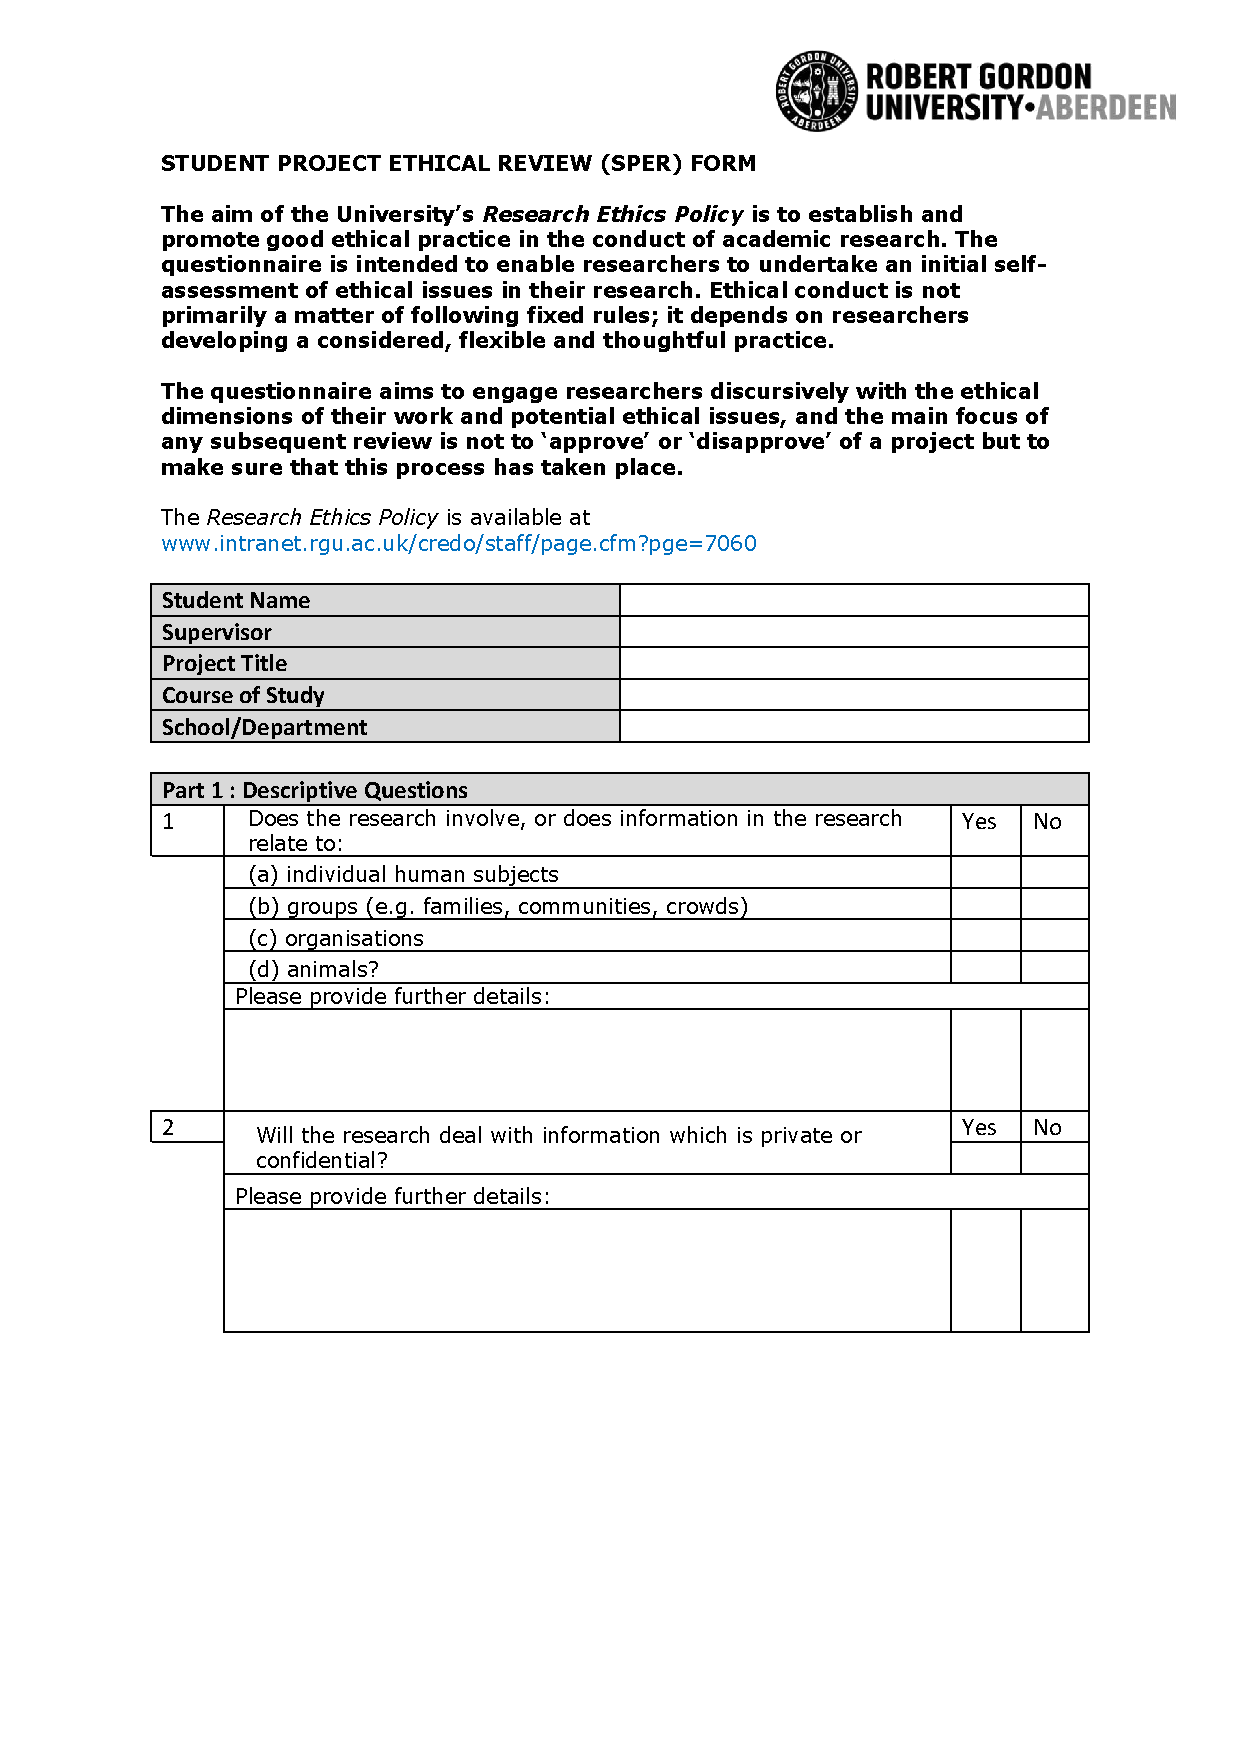
\includepdf[
    pages=-,
    fitpaper=true,
    pagecommand={}
]{EthicsForm.pdf}



% -------------------
% ABSTRACT
% -------------------
\chapter*{Abstract}
\addcontentsline{toc}{chapter}{Abstract}
Write your abstract here.

% -------------------
% PUBLICATION DETAILS
% -------------------
\chapter*{Publication Details}
\addcontentsline{toc}{chapter}{Publication Details}
Mention related publications here.

% -------------------
% ACKNOWLEDGEMENT
% -------------------
\chapter*{Acknowledgement}
\addcontentsline{toc}{chapter}{Acknowledgement}
Write your acknowledgements here.
\newpage
\tableofcontents
\newpage
\listoffigures
\newpage
\listoftables


\clearpage
\pagenumbering{arabic}
\setcounter{page}{1}
% -------------------
% MAIN CHAPTERS
% -------------------
\chapter{Introduction}

\section{Chapter Overview}
This chapter introduces the research study by outlining its main focus, context, and purpose. 
It provides a general overview of the topic, explains why it is important, and summarizes the structure of the introduction. 
The chapter also highlights how the research aligns with existing knowledge and sets the foundation for the following chapters.

\section{Problem Statement}
This section defines the central problem that the research aims to address. 
It clearly explains the gap or issue identified in the real world or within existing studies that motivates the need for this research. 
The problem statement should be concise, specific, and evidence-based, showing the reader why the issue is significant and worth investigating.

\section{Research Motivation}
This section explains the underlying reasons for conducting the study. 
It discusses the practical, theoretical, or personal motivations that led to the selection of the topic. 
The motivation may include current trends, societal or technological needs, or unresolved challenges found in previous work that inspired this investigation.

\section{Research Gap}
This section identifies the missing elements or limitations in the existing body of knowledge. 
It critically evaluates prior studies to show what has not yet been explored, adequately addressed, or empirically tested. 
Highlighting the research gap justifies the originality and necessity of the current study.

\section{Research Questions}
This section presents the key research questions that guide the study. 
Each question should align with the research problem and define the specific focus areas the study seeks to explore. 
Well-structured research questions help narrow the scope of the research and form the basis for analysis and discussion.

\section{Research Aim and Objectives}
This section defines the overall aim of the study and lists specific objectives designed to achieve it. 
The research aim should express the ultimate purpose of the study, while the objectives should break it down into clear, measurable, and achievable steps. 
These objectives should correspond directly to the research questions.

\section{Significance of the Research}
This section explains the importance and potential impact of the study. 
It discusses how the findings may contribute to academic knowledge, influence policy, or provide practical solutions. 
The section may also highlight who will benefit from the research (e.g., practitioners, researchers, organizations, or communities).

\section{Scope of the Research}
This section outlines the boundaries and limitations of the study. 
It defines the extent of the research in terms of subject area, population, data, tools, and timeframe. 
The scope helps clarify what is included and excluded, ensuring that the research remains focused and manageable.


\chapter{Literature Review}

\section{Chapter Overview}

This section provides an overview of the structure and purpose of the literature review. 
It outlines how previous studies, theories, and models are critically analyzed to build the foundation for the current research. 
The chapter identifies key themes, gaps, and debates relevant to the research problem, and highlights how the present study contributes to existing knowledge. 
It also explains the criteria used for selecting and organizing the reviewed literature.

\section{Background to the Problem}

This section introduces the broader context of the research problem. 
It discusses the theoretical and practical background that led to the identification of the issue under study. 
Relevant historical developments, key concepts, and domain-specific knowledge are summarized to help the reader understand why this problem is important. 
The section also establishes the link between the research topic and existing frameworks or theories, setting the stage for the detailed review that follows.
\section{Theoretical and Conceptual Background}

\section{Review of key methods and Technologies}


\section{Related Work}

This section critically examines previous research directly related to the study topic. 
It reviews existing models, methods, systems, and findings that have addressed similar problems or objectives. 
Key comparisons are drawn between different approaches, highlighting their strengths, weaknesses, and limitations. 
The discussion identifies research gaps that the current study aims to address. 
Where relevant, tables or diagrams may be used to summarize and contrast existing studies for clarity and organization. 

\noindent The section concludes by synthesizing the reviewed literature to demonstrate how the current research builds upon or diverges from prior work, thereby justifying the need for this study.


\chapter{Methodology}
\section{Chapter Overview}
Provide an overview of the chapter and the purpose. Brief the outline of the chapter contents.

\section{Research Methodology}

Identify the research methodology that you follow in your study and give a brief justification on each choice. 

\section{any related sub sections you have}

\chapter{Any other Chapters as required}

\chapter{Results}

\section{Chapter Overview}
This chapter presents the findings of the study based on the data collected and analyzed using the methods described in the previous chapter. 
It provides both quantitative and qualitative results, supported by appropriate figures, tables, and charts where relevant. 
The purpose of this chapter is to present the results objectively without interpretation, ensuring that the data directly reflects the outcomes of the research questions or hypotheses.


\chapter{Discussion}

\section{Chapter Overview}
This chapter interprets and explains the significance of the results presented in the previous chapter. 
It connects the findings to the research questions, objectives, and existing literature. 
The discussion highlights whether the outcomes support or contradict prior studies and offers possible explanations for any unexpected results. 
It emphasizes the theoretical, practical, and methodological implications of the findings.
\section{Any relevant sub sections}



\chapter{Conclusion}

\section{Summary}
This section provides a concise summary of the entire research project. 
It restates the research aim, objectives, and key findings while emphasizing how these findings address the research problem. 
The summary also reflects on the overall contribution of the study to existing knowledge and practice.

\section{Limitations}
This section discusses the constraints or weaknesses encountered during the research. 
Limitations may include issues such as sample size, data accessibility, time constraints, methodological boundaries, or assumptions made during analysis. 
Acknowledging these limitations enhances the transparency and credibility of the study.

\section{Future Work}
This section proposes directions for future research based on the findings and limitations of the current study. 
It suggests how future studies could build upon this work, overcome identified challenges, or explore new dimensions of the problem. 
The section encourages continued investigation to expand knowledge and improve applications in the research field.

\section{Reflective Report}
This section provides a personal reflection on the research process, challenges faced, and lessons learned throughout the study. 
It discusses how the research experience contributed to academic and professional development, problem-solving skills, and subject-matter understanding. 
The reflection may also include commentary on data collection experiences, time management, ethical considerations, and areas for personal improvement in future research.

% -------------------
% REFERENCES
% -------------------
\addcontentsline{toc}{chapter}{References}
\bibliographystyle{apalike} % or Harvard
\bibliography{references}

% -------------------
% APPENDICES
% -------------------
\appendix
\chapter*{Appendix}

\end{document}
```
